\section{Training Setup}
In Fig. \ref{fig:teaser2}, we compare the training setup for the cross-entropy, self-supervised contrastive and supervised contrastive (SupCon) losses. Note that the number of parameters in the inference models always stays the same.  We also note that it is not necessary to train a linear classifier in the second stage, and previous works have used k-Nearest Neighbor classification \cite{wu2018unsupervised} or prototype classification to evaluate representations on classification tasks. The linear classifier can also be trained jointly with the encoder, as long as it doesn't propagate gradients back to the encoder. 

\begin{figure}[h]  
 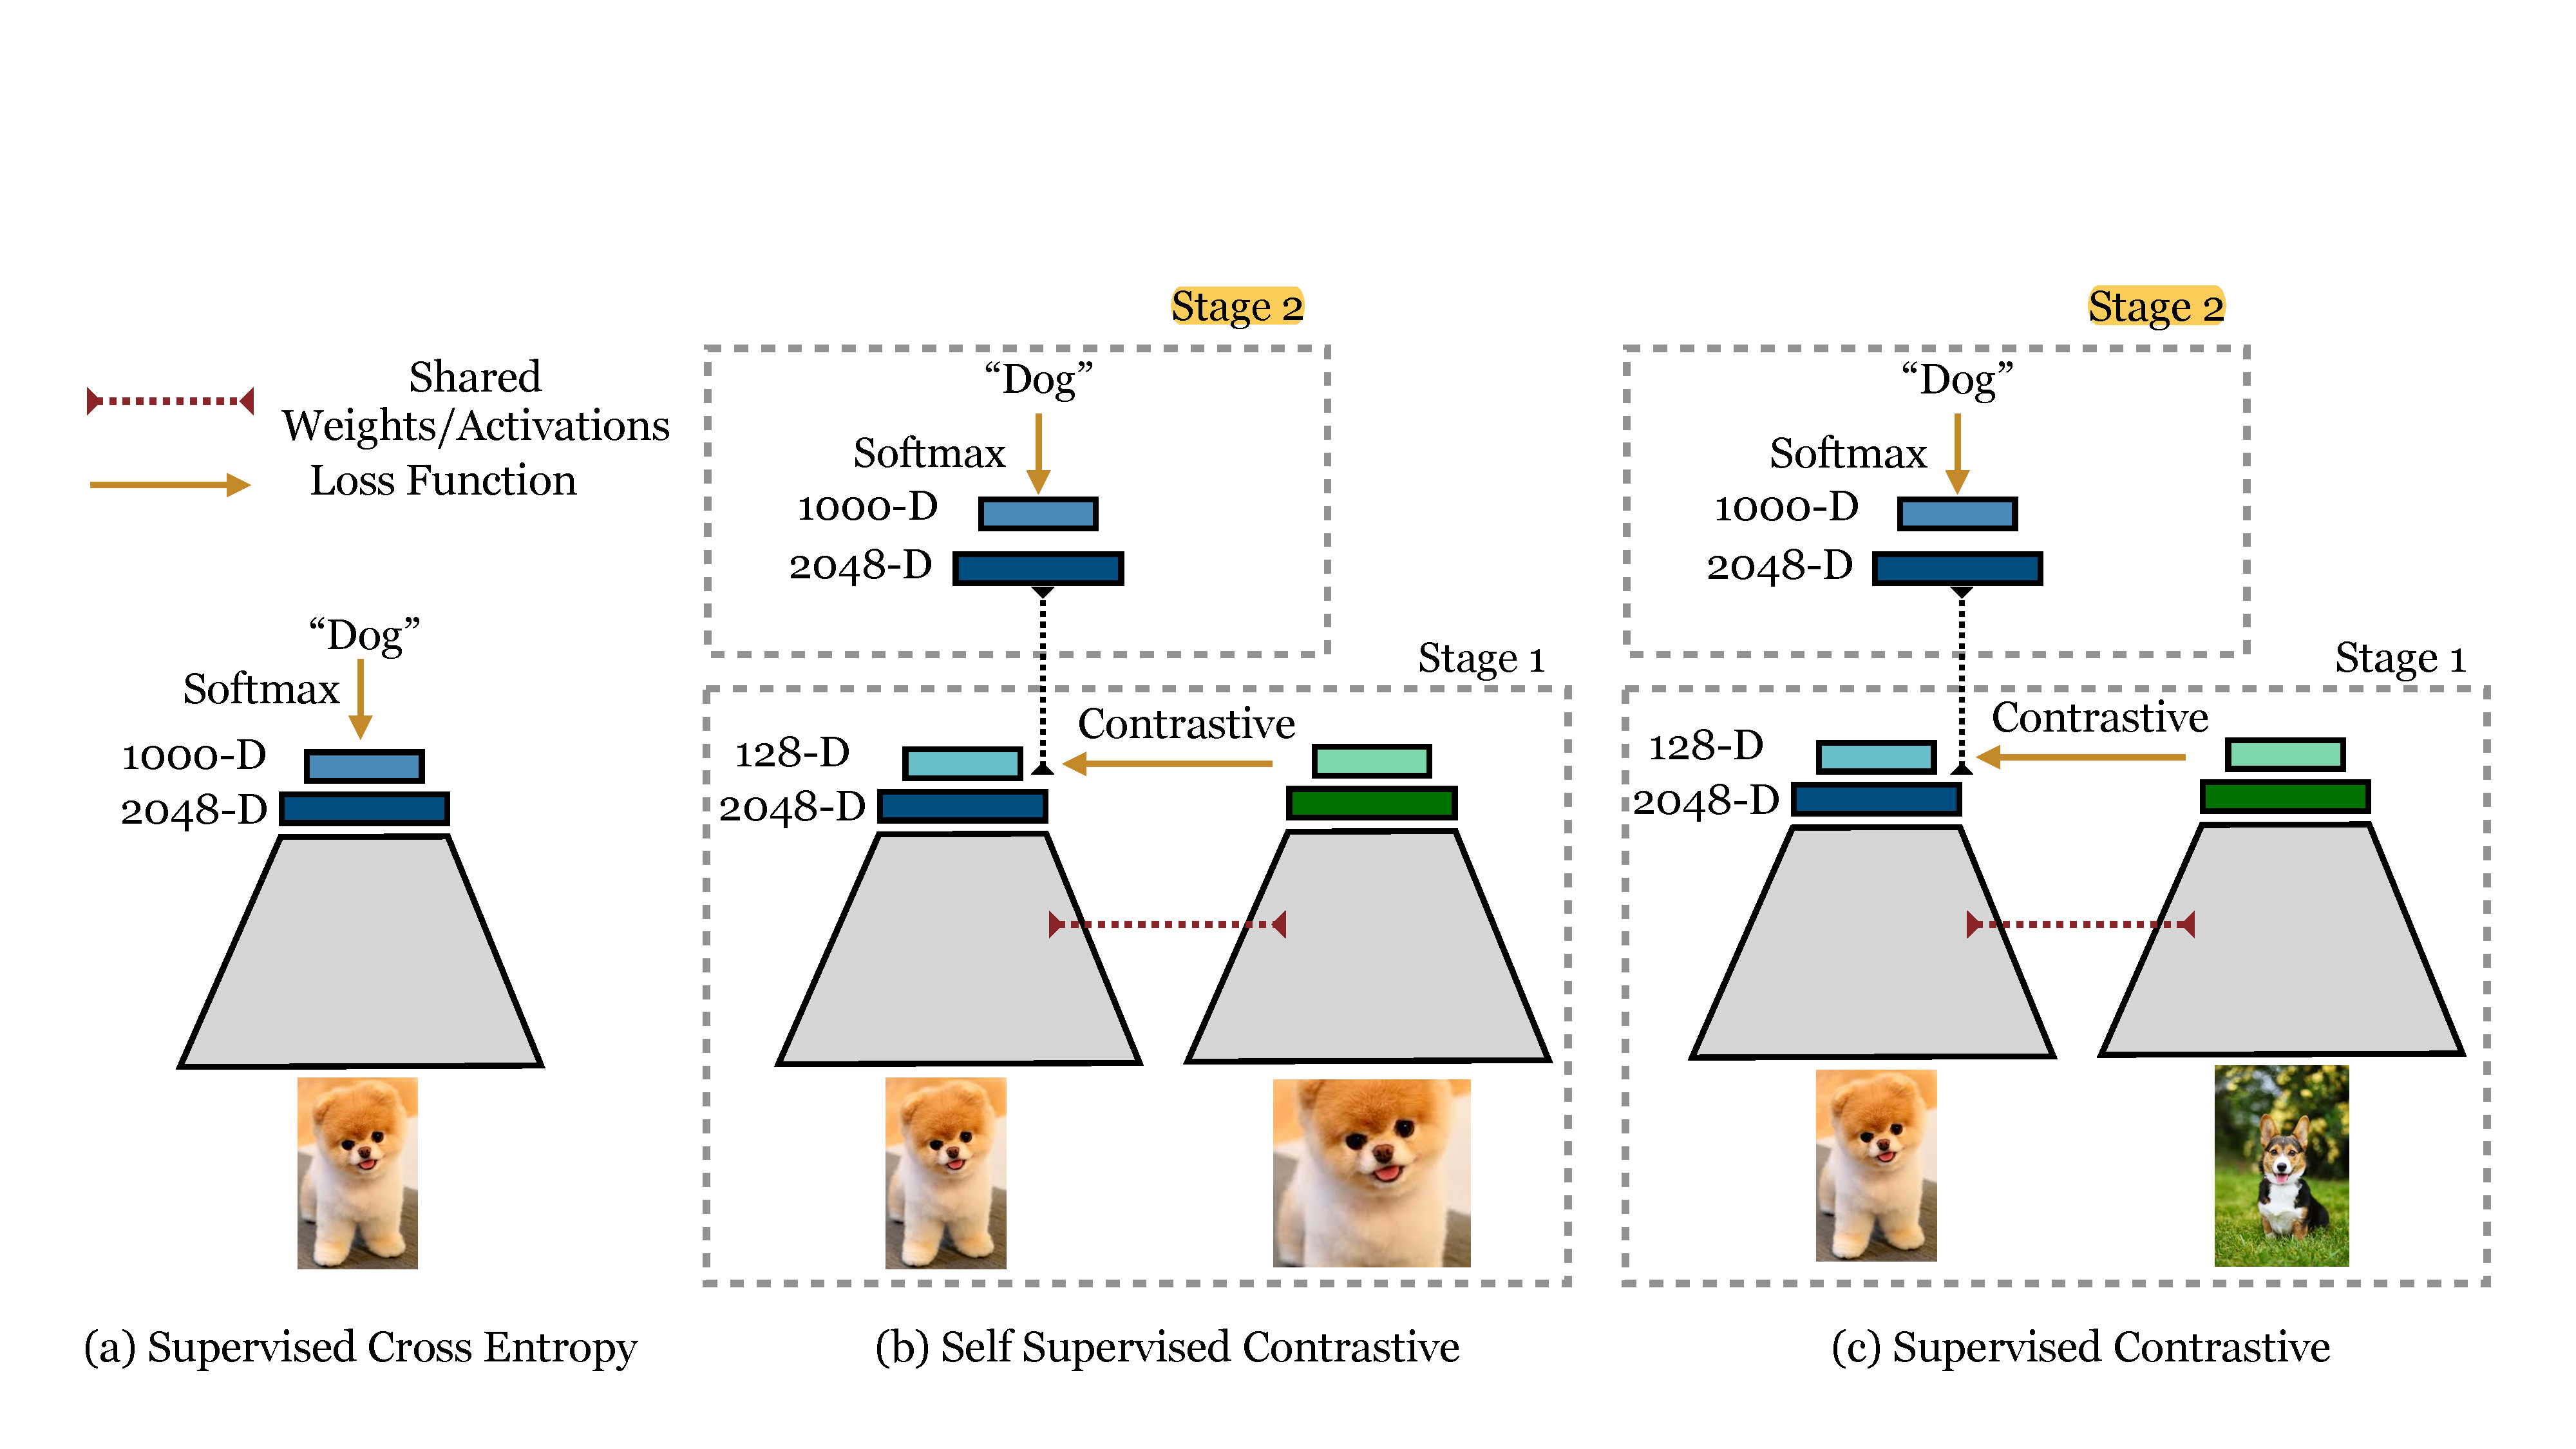
\includegraphics[width=\linewidth]{./figs/teaser_new2}
  \caption{Cross entropy, self-supervised contrastive loss and supervised contrastive loss: The cross entropy loss (left) uses labels and a softmax loss to train a classifier; the self-supervised contrastive loss (middle) uses a contrastive loss and data augmentations to learn representations. The supervised contrastive loss (right) also learns representations using a contrastive loss, but uses label information to sample positives in addition to augmentations of the same image. Both contrastive methods can have an optional second stage which trains a model on top of the learned representations. }
  \label{fig:teaser2}
\end{figure}

